\chapter{Trabalhos Relacionados}
\label{trabalhos}

Como forma de elencar soluções similares e trabalhos relacionados, alguns trabalhos, em conjunto com outros identificados no processo descrito na Seção \ref{fundamentacao:ageis:fatores}, foram investigados. Nesses trabalhos, são abordados métodos para avaliar a qualidade do TE, além da importância de garantir a alta qualidade desse fator.

Em \cite{moe}, os autores propõem uma ferramenta que, segundo eles, contempla aspectos e características essenciais, apresentados em cinco dimensões (i.e., \textit{Liderança Compartilhada}, \textit{Orientação da Equipe}, \textit{Redundância}, \textit{Aprendizagem da Equipe} e \textit{Autonomia da Equipe}) que precisam ser abordadas para garantir a alta qualidade do TE. Os conceitos dessas dimensões estão apresentados na Tabela \ref{fundamentacao:ageis:fatores:tabela}. Os resultados do instrumento são apresentados em um gráfico de radar, que representa o status atual do TE. Como forma de avaliar a qualidade do TE, foi definida uma pergunta pra cada dimensão abordada pela ferramenta. As perguntas devem ser respondidas em uma escala que vai de 0 à 10, onde os limites dessa escala são descritos para facilitar a resposta dessas perguntas por parte dos usuários. Essa ferramenta também é utilizada em \cite{ringstad}.

De acordo com os autores, pesquisadores e pessoas que atuam na indústria reconhecem que as cinco dimensões abordadas pela ferramenta são essenciais para o TE em ambientes ágeis. Além disso, a ferramenta é apropriada para verificar mudanças na qualidade do TE ao longo do tempo. Entretanto, essa abordagem não considera outros fatores essenciais que influenciam a qualidade do TE. Além disso, o gráfico de radar que contém o status atual do TE não provê informações objetivas acerca do estado atual do TE.

Hoegl et al. \cite{hoegl} conceitualizam a qualidade do TE como a qualidade das interações entre os membros de um time. Os autores propõem seis características indicadoras de colaboração no trabalho, e as combinam como fatores determinantes para a qualidade do TE. Essas seis características são: \textit{Comunicação}, \textit{Coordenação}, \textit{Balanço da Contribuição dos Membros}, \textit{Suporte Mútuo}, \textit{Esforço} e \textit{Coesão}.

Nesse trabalho, a principal proposição dos autores é a de que a qualidade do TE está positivamente relacionada com o sucesso de projetos inovadores. Foram realizadas entrevistas com o intuito de coletar dados de equipes de desenvolvimento, gerentes de projeto e gerentes que não são parte da equipe para avaliar a veracidade dessa proposição. Nessas entrevistas, os indivíduos responderam perguntas relacionadas aos seis fatores que influenciam a qualidade do TE, e deram suas opiniões à respeito do sucesso de seus projetos. Com base nos resultados, os autores concluíram que o desempenho da equipe é positivamente influenciado pela qualidade do TE.

Entretanto, o conceito de qualidade do TE atrelado aos seis fatores descritos por Hoegl et al. \cite{hoegl} correspondem apenas ao grau colaboração da equipe, não contemplando outros fatores como, (e.g., \textit{Autonomia da Equipe}). Além disso, apesar do contexto de projetos inovadores ser similar ao de projetos ágeis \cite{freire}, em \cite{hoegl} não há informações relacionadas às metodologias utilizadas nos projetos em que os indivíduos entrevistados trabalharam.

Em \cite{amengual} é apresentado um modelo de referência para avaliação do TE em equipes de desenvolvimento de \textit{software}, além de um processo para utilizar esse modelo e um \textit{framework} para efetuar a medição. O modelo utilizado como base para essa avaliação proposta considera quatro fatores relacionados ao TE: \textit{Gerenciamento}, \textit{Composição}, \textit{Comunicação} e \textit{Motivação}. Para utilizar o modelo, foram elaboradas perguntas que compõem um questionário para cada um desses fatores.

De acordo com os autores, apesar do TE ter sido analisado e discutido na literatura por muitos anos, não existia um \textit{framework} que poderia ser utilizado como referência para avaliar a qualidade do TE no contexto de desenvolvimento de \textit{software}. Portanto, eles sugerem que o \textit{framework} proposto pode ser utilizado como referência.

Contudo, como o trabalho apresentado em \cite{amengual} é voltado pra equipes de desenvolvimento de \textit{software} em geral, o modelo de referência não contempla vários aspectos essenciais de equipes ágeis. Além disso, assim como em \cite{moe} e \cite{hoegl}, não fica explícito como a combinação dos resultados referentes aos fatores-chave do TE determina a qualidade do aspecto principal, que é o \textit{Trabalho em Equipe}.

\section{Trabalho Base}
\label{trabalhos:base}

Esta pesquisa tem como base o trabalho apresentado em \cite{freire}. Nesse trabalho, a necessidade de avaliar a qualidade do TE é apresentada, e um modelo baseado em RB é proposto para realizar essa avaliação. O conceito de qualidade do TE, nesse trabalho, é considerado como a união da eficiência da colaboração, do gerenciamento das atividades e dos atributos da equipe - atributos pessoais dos membros da equipe e o expertise deles.

O modelo proposto em \cite{freire} foi construído tomando como base apenas o trabalho de Hoegl et al. \cite{hoegl}. As modificações feitas no modelo base foram feitas com ajuda de especialistas em entrevistas individuais. Após as modificações, a versão final do modelo proposto em \cite{freire} ficou como representado na Figura \ref{trabalho:base:modelo}.

\begin{figure}[ht!]
\begin{center}
        \fbox{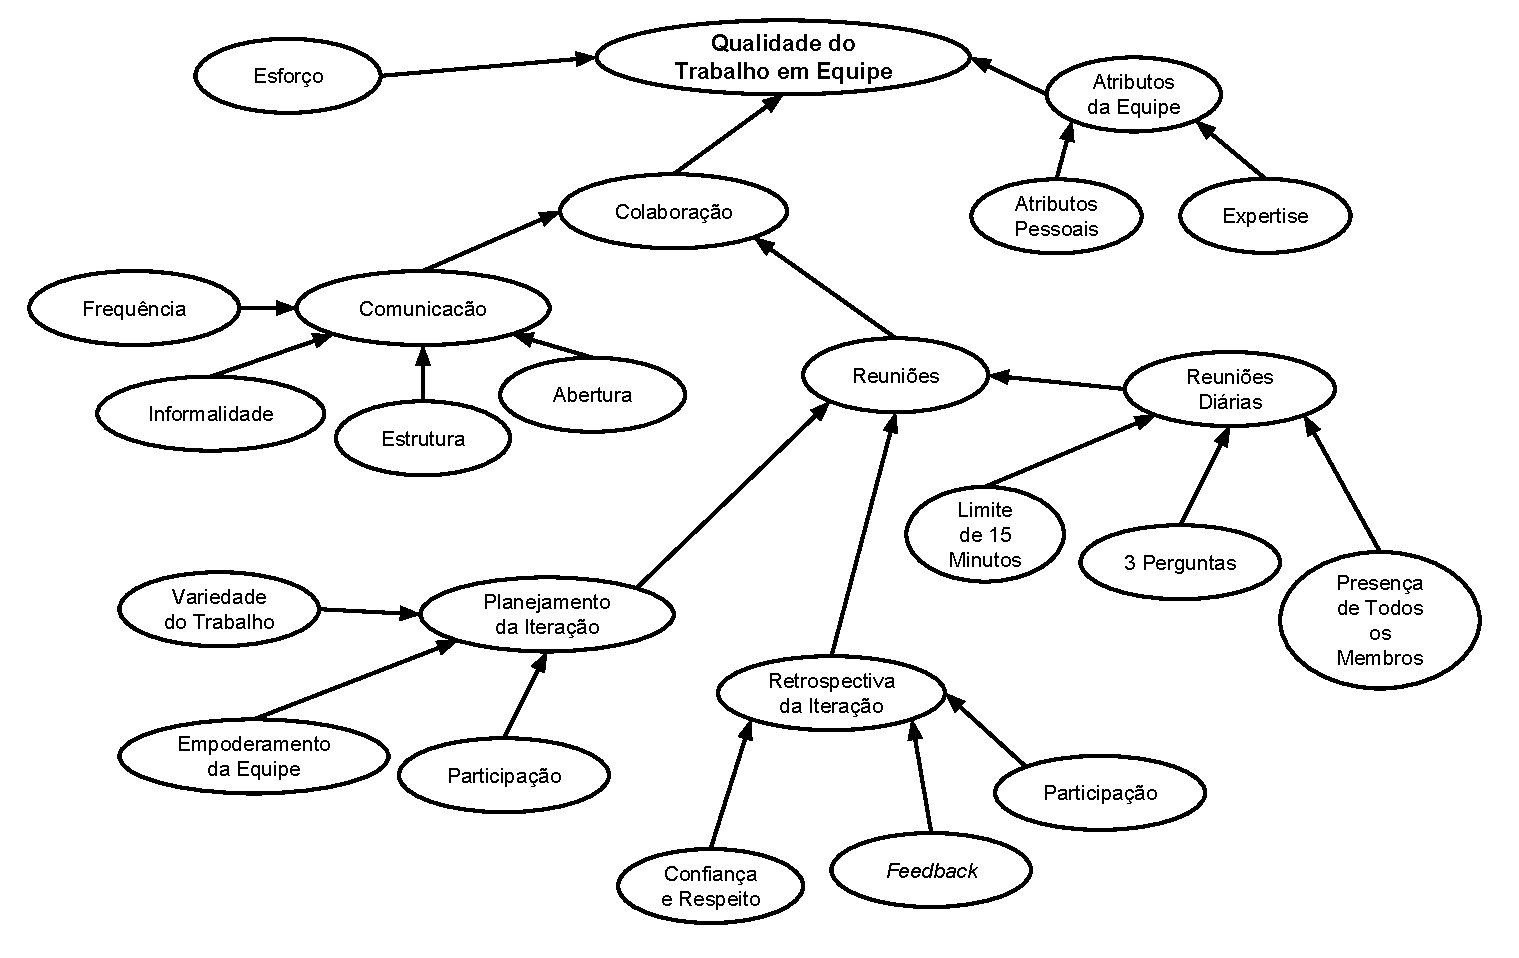
\includegraphics[scale=0.6]{figs/modeloSBES.pdf}}
    \end{center}
    \caption{Modelo Proposto no Trabalho Base}
    \label{trabalho:base:modelo}
\end{figure}

As tabelas de probabilidade desse modelo foram definidas utilizando o método de \cite{perkusichNPT}. Contudo, em vez de utilizar \textit{surveys} online, foram realizadas entrevistas com o mesmos especialistas responsáveis por construir o GAD. Para cada nó filho presente no GAD, pediu-se que os especialistas ordenassem seus nós pai com base na sua relevância para o nó filho. Em seguida, com base nessas ordens de relevância foram definidas as expressões ponderadas para, finalmente, definir as TPN dos nós filho.

A validação desse modelo foi feita com simulação de cenários, e, de acordo com as conclusões, o modelo é uma boa representação do mundo real. Além disso, também foi concluído que o modelo permite que, baseado nos resultados do modelo, os indivíduos que o utilizam identifiquem problemas que compromentem a qualidade do TE. Entretanto, há alguns fatores que afetam a sua validade:

\begin{itemize}
  \item A utilização de apenas um trabalho como base para a construção do modelo;
  \item A definição das TPN utilizando o método de Perkusich et al. utiliza apenas a função de média ponderada. Logo, as TPN de alguns nós podem estar inconsistentes pelo fato de sua definição ser restrita à essa função;
  \item O modelo não foi validado em projetos reais.
\end{itemize}

Portanto, nesta pesquisa, foi dada continuidade ao trabalho apresentado em \cite{freire}, buscando eliminar esses fatores que ameaçaram a sua validade.
